\documentclass[french]{article}
\usepackage[T1]{fontenc}
\usepackage[utf8]{inputenc}
\usepackage{lipsum}
\usepackage{lmodern}
\usepackage{geometry}
\usepackage{babel}
\usepackage{graphicx}
\usepackage{lastpage}
\usepackage{ragged2e}
\usepackage{enumitem}
\usepackage[normalem]{ulem}
\usepackage{hyperref} % pour \url{URL}
\usepackage{color} % pour \textcolor{color}{text}
\usepackage{listings} % pour afficher du code
\usepackage{longtable} % pour l'environnement longtable
\usepackage{float} % pour des figures non flottantes

% Grammaire EBNF
\usepackage{syntax}
\setlength{\grammarparsep}{5pt plus 1pt minus 1pt}
\setlength{\grammarindent}{11em}

% Diagramme de flux
\usepackage{tikz}
\usetikzlibrary{shapes,arrows}
\tikzstyle{decision} = [diamond, draw, fill=green!20, text width=5em, text badly centered, inner sep=0pt]
\tikzstyle{block} = [rectangle, draw, fill=blue!20, text width=6em, text centered, rounded corners, minimum height=4em]
\tikzstyle{line} = [draw, -latex']
\tikzstyle{cloud} = [draw, ellipse,fill=red!20, minimum height=2em]

% Style C++
\lstset{
	language=C++,
	tabsize=2,
	basicstyle=\ttfamily,
	keywordstyle=\color{blue}\ttfamily,
	stringstyle=\color{red}\ttfamily,
	commentstyle=\color{black!40}\ttfamily,
	morecomment=[l][\color{black!50}]{\#},
	gobble=8
}

\geometry{
	a4paper,
	total={210mm,297mm},
	left=20mm,
	right=20mm,
	top=20mm,
	bottom=20mm,
}

\usepackage{fancyhdr}
\pagestyle{fancy}
\setlist[enumerate,1]{leftmargin=2cm}

% Entêtes
\lhead{Browne Champion Djomo Hardy Richoz Rochat}
\chead{}
\rhead{PRO}
\renewcommand{\headrulewidth}{0.4pt}
\renewcommand{\footrulewidth}{0.4pt}

\begin{document}
	
	% Titre du document
	\title{GraphY} % ou un autre nom
	\author{Rapport\\ 
		Projet de semestre\\
		Browne Champion Djomo Hardy Richoz Rochat\\
		Resp. René Rentsch\\
		HEIG-VD}
	\date{\today} % date du jour
	\maketitle
	
	% Tables des matières
	\tableofcontents
	
	% Tables des figures
	\listoffigures
	
	% Pour tout le document
	\justify
	\normalsize
	
	\section{Cadre de développement} 
		L'application est développée à l'aide du langage C++ et de la bibliothèque Qt \textcolor{red}{(insérer les versions utilisées ainsi que les compilateurs ?)}. Afin que le code source soit écrit dans le même style par tous les membres du groupe, nous avons décider d'utiliser le Coding Style de Qt qui correspond bien à nos besoins: \url{https://wiki.qt.io/Qt_Coding_Style}.
			
	\section{Interpréteur} % Champion
		Dans le cadre de l'application, l'utilisateur est amené à entrer des commandes lui permettant de créer et de modifier des graphes, tout autant que d'appeler des fonctions effectuant différents traitements (algorithmes, lecture depuis un fichier, ...). 
	
		\subsection{Normalisation du langage} 
			Il est nécessaire de définir une grammaire claire sur la syntaxe des commandes, ainsi que leur sémantique.
			
			\subsubsection{Analyse des types et des opérations} 
				Premièrement, il faut définir les types disponibles dans le langage. Pour cela il est intéressant de partir des algorithmes de graphe et de voir les types de résultats que nous attendons en sortie, ainsi que les types de paramètres dont nous aurons besoin:
			
				\begin{itemize}
					\item Boolean: un graphe a-t-il un cycle? est-il eulérien? ...
					\item Number: poids d'un arc, indice d'un sommet, ...
					\begin{itemize}
						\item Integer: pour les index, ...
						\item Float: pour les poids, ...
					\end{itemize}
					\item String: label d'un sommet, nom d'une fonction, ...
					\item Array: liste d'arêtes, matrices (Floyd-Warshall), ...
					\item Graph: le graphe à proprement parler
					\begin{itemize}
						\item Vertex: un sommet, son indice, son poids, ...
						\item Edge: une arête/arc, son poids, ...
					\end{itemize}
				\end{itemize} 
			
				Puisque nous avons à présent une idée des types disponibles, il faut définir leur domaine ainsi que les opérations disponibles et leur syntaxe. On fait le choix délibéré de se concentrer sur les opérations concernant les graphes, les opérations simples comme additionner deux nombres où les comparaisons ne sont pas prévues. Cependant la base du langage doit permettre de les définir plus tard. 
			
				\begin{longtable}{lll}
					\textbf{\texttt{Boolean}}\\ \hline \hline
					Domaine & \multicolumn{2}{l}{\texttt{True} ou \texttt{False}}\\ 
					Opérations & Déclaration & \texttt{Boolean a = True;}\\
					& Affectation & \texttt{a = False; a = f();}\\
					& Lecture & \texttt{a; f(a); Boolean b = a;}\\ 
					\\
					\textbf{\texttt{Number}}\\ \hline \hline
					Domaine & \multicolumn{2}{l}{\texttt{Integer} et \texttt{Float}}\\ 
					\\
					\textbf{\texttt{Integer}}\\ \hline \hline
					Domaine & \multicolumn{2}{l}{Entier signé sur 32 bits}\\
					Opérations & Déclaration & \texttt{Integer a = -20;}\\
					& Affectation & \texttt{a = 2; a = f();}\\
					& Lecture & \texttt{a; f(a); Integer b = a;}\\ 
					\\
					\textbf{\texttt{Float}}\\ \hline \hline
					Domaine & \multicolumn{2}{l}{Nombre à virgule flottante sur 32 bits}\\
					Opérations & Déclaration & \texttt{Float a = -32.4;}\\
					& Affectation & \texttt{a = 4.0; a = f();}\\
					& Lecture & \texttt{a; f(a); Float b = a;}\\ 
					\\
					\textbf{\texttt{String}}\\ \hline \hline
					Domaine & \multicolumn{2}{l}{Ensemble de zéro ou plusieurs caractères ASCII}\\
					Opérations & Déclaration & \texttt{String a = "Hello";}\\
					& Affectation & \texttt{a = "World"; a = f();}\\
					& Lecture & \texttt{a; f(a); String b = a;}\\ 
					\\
					\textbf{\texttt{Array}}\\ \hline \hline
					Domaine & \multicolumn{2}{l}{Tableau dynamique hétérogène}\\
					Opérations & Déclaration & \texttt{Array a = [1.0, "Salut", 3];}\\
					& Affectation & \texttt{a = [4, 5];}\\ 
					& Lecture & \texttt{a; f(a); Array b = a;}\\
					& Accès & \texttt{Integer c = a[1];}\\ 
					\\
					\textbf{\texttt{Vertex}}\\ \hline \hline
					Domaine & \multicolumn{2}{l}{Sommet avec des informations supplémentaires facultatives}\\
					Opérations & Déclaration & \texttt{Vertex a = (1); Vertex a2 = (2::3);}\\
					& & \texttt{(id:label:weight:max\_capacity:min\_capacity)}\\
					& Affectation & \texttt{a = (1:"Yverdon"); a = f();}\\
					& Lecture & \texttt{a; f(a); Vertex b = a;}\\ 
					\\
					\textbf{\texttt{Edge}}\\ \hline \hline
					Domaine & \multicolumn{2}{l}{Arête/arc avec des informations supplémentaires facultatives}\\
					Opérations & Déclaration & \texttt{Edge a = (1--2); Edge a2 = (2<-3:5);}\\
					& & \texttt{(connection[id]:weight:label:max\_capacity:min\_capacity)}\\
					& & \texttt{(arête: -- (tiret double) arcs: ->, <-)}\\
					& Affectation & \texttt{a = (1->2::"A1"); a = f();}\\
					& Lecture & \texttt{a; f(a); Vertex b = a;}\\ 
					\\
					\textbf{\texttt{Graph}}\\ \hline \hline
					Domaine & \multicolumn{2}{l}{Ensemble de sommets et d'arêtes/arcs (les parenthèses ne sont plus obligatoires)}\\
					Opérations & Déclaration & \texttt{Graph a = \{0, 1, 2:A, 1->2:3:::2]\};}\\
					& & (si on ne veut pas écrire tous les sommets: \texttt{a = \{\#3, 0->1, 0->2\};})\\
					& Affectation & \texttt{a = \{0, 1, 0--1\}; a = f();}\\
					& Lecture & \texttt{a; f(a); Graph b = a;}\\
					& Ajout/modification & \texttt{a += (1<-2:4)};\\
					& Suppression & \texttt{a -= [(3), (1->2)];}\\
				\end{longtable}
				
				Ce tableau nous donne à présent une vue assez claire de nos besoins, cependant certaines opérations des types complexes (\texttt{Array, Vertex, Edge} et \texttt{Graph}) méritent d'être approfondies:
				
				\begin{itemize}
					\item \texttt{Array}: 
					\begin{itemize}
						\item Index de 0 à n-1
						\item Accès en dehors des bornes $\rightarrow$ Exception
					\end{itemize}
					\item \texttt{Vertex}:
					\begin{itemize}
						\item Seul le premier paramètre (\texttt{id[Integer]}) est obligatoire, et il ne doit pas être négatif
						\item Les valeurs par défaut sont \texttt{label[String]="", weight[Number]=0, max\_capacity[Number]=min\_capacity, min\_capacity[Number]=0}
					\end{itemize}
					\item \texttt{Edge}: 
					\begin{itemize}
						\item Seul le premier paramètre (\texttt{connection}) est obligatoire
						\item Le paramètre \texttt{id[Integer]} doit être positif ou nul et sa valeur par défaut est 0
						\item Les valeurs par défaut sont \texttt{weight[Number]=0, label[String]="", max\_capacity[Number]=min\_capacity, min\_capacity[Number]=0}
						\item L'\texttt{id} est un identifiant "local" à la \texttt{connection}
					\end{itemize}
					\item \texttt{Graph}: 
					\begin{itemize}
						\item La création d'un graphe vide est permis (\texttt{Graph g = \{\};})
						\item Le raccourci d'écriture pour le nombre de sommet (\texttt{\#3}) doit se trouver au début
						\item Pour que le \texttt{Vertex} d'\texttt{id n} soit créé, il faut que tous les \texttt{id} de \texttt{0} à \texttt{n-1} existent déjà, sinon $\rightarrow$ Exception 
						\item Dans le cas d'arêtes/arcs multiples, par exemple \texttt{\{\#2, 0->1, 0->1\}}, le paramètre \texttt{id} du second \texttt{Edge} est incrémenté $\rightarrow$ \texttt{0->1[0]} et \texttt{0->1[1]}
						\item Pour qu'un \texttt{Edge} soit créé, il est nécessaire que les deux \texttt{Vertex} soit déjà créés, sinon $\rightarrow$ Exception
						\item Ajouts / modifications:
						\begin{itemize}
							\item Les types acceptés en opérande de droite sont \texttt{Vertex, Edge} ou un \texttt{Array} de ces deux types
							\item Pour les \texttt{Vertex}, si l'\texttt{id} existe déjà dans le graphe, c'est une modification, sinon c'est un ajout
							\item Pour les \texttt{Edge}, si la \texttt{connection} existe déjà dans le graphe mais que l'\texttt{id} est omis, alors c'est un ajout, sinon c'est une modification (sauf si l'\texttt{id} n'existe pas, dans ce cas c'est un ajout)
							\item La modification est accumulative, par exemple si on fait \texttt{Graph g = \{0:"Yverdon"\}; g += (0::2);}, alors le \texttt{Vertex} résultant est \texttt{(0:"Yverdon":2)}
						\end{itemize}
						\item Suppressions:
						\begin{itemize}
							\item Les types acceptés en opérande de droite sont \texttt{Vertex, Edge} ou un \texttt{Array} de ces deux types
							\item S'il n'y a rien à supprimer, alors il ne se passe rien (pas d'exception)
							\item La suppression d'un \texttt{Vertex} entraine la suppression des \texttt{Edge} associés
							\item Pour les \texttt{Edge}, si l'\texttt{id} est omis, alors toutes les \texttt{connection} sont supprimées
						\end{itemize}
					\end{itemize}
				\end{itemize}
				
				Notons que les erreurs sont gérées au travers d'exceptions.\\
				
				Maintenant que les types des variables et leurs opérations de base sont définis, on veut pouvoir effectuer d'autres traitements sur ces variables (ajouter une nouvelle opération ou appliquer un algorithme). Cela va se faire via des fonctions prédéfinies (la définition de fonction n'est pas prévue).\\
				
				Prototype d'une fonction: \texttt{R f(T1, T2, ...);} avec \texttt{R} le type de retour, \texttt{f} le nom de la fonction et \texttt{Tn} le type du paramètre en position \texttt{n}.\\
				
				Appel d'une fonction: \texttt{Graph a = dijkstra(g, 1);} ou \texttt{g = removeAllPonderation(g);}.\\
				
				Le passage des paramètres se fait par copie (ou référence constante) et la correspondance est par position. On autorise la surcharge des fonctions.
			
			\subsubsection{Grammaire EBNF} 
				L'analyse étant finie, on peut à présent développer les règles de production EBNF du langage. On part des règles de haut niveau pour descendre dans la hiérarchie (inspiration: \url{http://www.fit.vutbr.cz/study/courses/APR/public/ebnf.html}).\\
				
				\textbf{Point de départ (entrée utilisateur)}
				\begin{grammar}
					<start> ::= <statement> \{ <statement> \}
				\end{grammar}
				
				\textbf{Déclarations (statements)}
				\begin{grammar}
					<statement> ::= ( <function-call> | <declaration> | <assignment> ) \lit{;}
					
					<function-call> ::= <identifier> <parameter-list>
					
					<declaration> ::= <type> <identifier> \lit{=} <parameter>
					
					<assignment> ::= <variable> \lit{=} <parameter>
					
					<parameter-list> ::= \lit{(} <parameter> \{ \lit{,} <parameter> \} \lit{)}
					
					<parameter> ::= <constant> | <indexed-array> | <function-call>
				\end{grammar}
				
				\textbf{Expressions et opérations}
				\begin{grammar}
					<indexed-array> ::= <variable> \lit{[} <digit-sequence> \lit{]}
				\end{grammar}
				
				\textbf{Types de variable et d'enregistrement}
				\begin{grammar}
					<type> ::= <simple-type> | <complex-type>
					
					<simple-type> ::= \lit{Boolean} | \lit{Number} | \lit{Integer} | \lit{Float} | \lit{String}
					
					<complex-type> ::= \lit{Array} | \lit{Graph} | \lit{Vertex} | \lit{Edge}
					
					<array-record> ::= \lit{[} <constant> \{ \lit{,} <constant> \} \lit{]}
					
					<constant> ::= <simple-constant> | <complex-constant>
					
					<complex-constant> ::= <array-record> | <graph-record> | <edge-record> | <vertex-record>
					
					<graph-record> ::= \lit{\{} <graph-info> \{ \lit{,} <graph-info> \} \lit{\}}
					\alt \lit{\{} \lit{\#} <digit-sequence> \{ \lit{,} <graph-info> \} \lit{\}}
					
					<edge-record> ::= \lit{(} <edge-info> \lit{)}
					
					<vertex-record> ::= \lit{(} <vertex-info> \lit{)}
					
					<graph-info> ::= <vertex-info> | <edge-info>
					
					<edge-info> ::= <connection> 
					\alt <connection> \lit{:} <number>
					\alt <connection> \lit{:} [ <number> ] \lit{:} <string>
					\alt <connection> \lit{:} [ <number> ] \lit{:} [ <string> ] \lit{:} <number>
					\alt <connection> \lit{:} [ <number> ] \lit{:} [ <string> ] \lit{:} [ <number> ] \lit{:} <number>
					
					<vertex-info> ::= <id> 
					\alt <id> \lit{:} <string>
					\alt <id> \lit{:} [ <string> ] \lit{:} <number>
					\alt <id> \lit{:} [ <string> ] \lit{:} [ <number> ] \lit{:} <number>
					\alt <id> \lit{:} [ <string> ] \lit{:} [ <number> ] \lit{:} [ <number> ] \lit{:} <number>
					
					<connection> ::= <id> ( \lit{\textendash\textemdash} | \lit{\textemdash\textgreater} | \lit{\textless\textemdash} ) <id>
					
					<id> ::= <digit-sequence>
				\end{grammar}
				
				\textbf{Identifiants et définitions de bas niveau}
				\begin{grammar}
					<simple-constant> ::= <sign> <variable> | <number> | <boolean> | <string>
					
					<variable> ::= <identifier>
					
					<identifier> ::= <letter> \{ <letter> | <digit> | \lit{\_} \}
					
					<string> ::= \lit{"\""} \{ <letter> | \lit{ } \} \lit{"\""}
					
					<letter> ::= ? all lower and upper case letters ? 
					
					<boolean> ::= \lit{True} | \lit{False}
					
					<number> ::= <integer-number> | <real-number>
					
					<real-number> ::= [ <sign> ] <digit-sequence> \lit{.} <digit-sequence>
					
					<integer-number> ::= [ <sign> ] <digit-sequence>
					
					<digit-sequence> ::= <digit> \{ <digit> \}
					
					<sign> ::= \lit{+} | \lit{-} 
					
					<digit> ::= ? all digits from 0 to 9 ? 
				\end{grammar}
		
		\subsection{Flux des données}
			\begin{figure}[H]
				\centering
				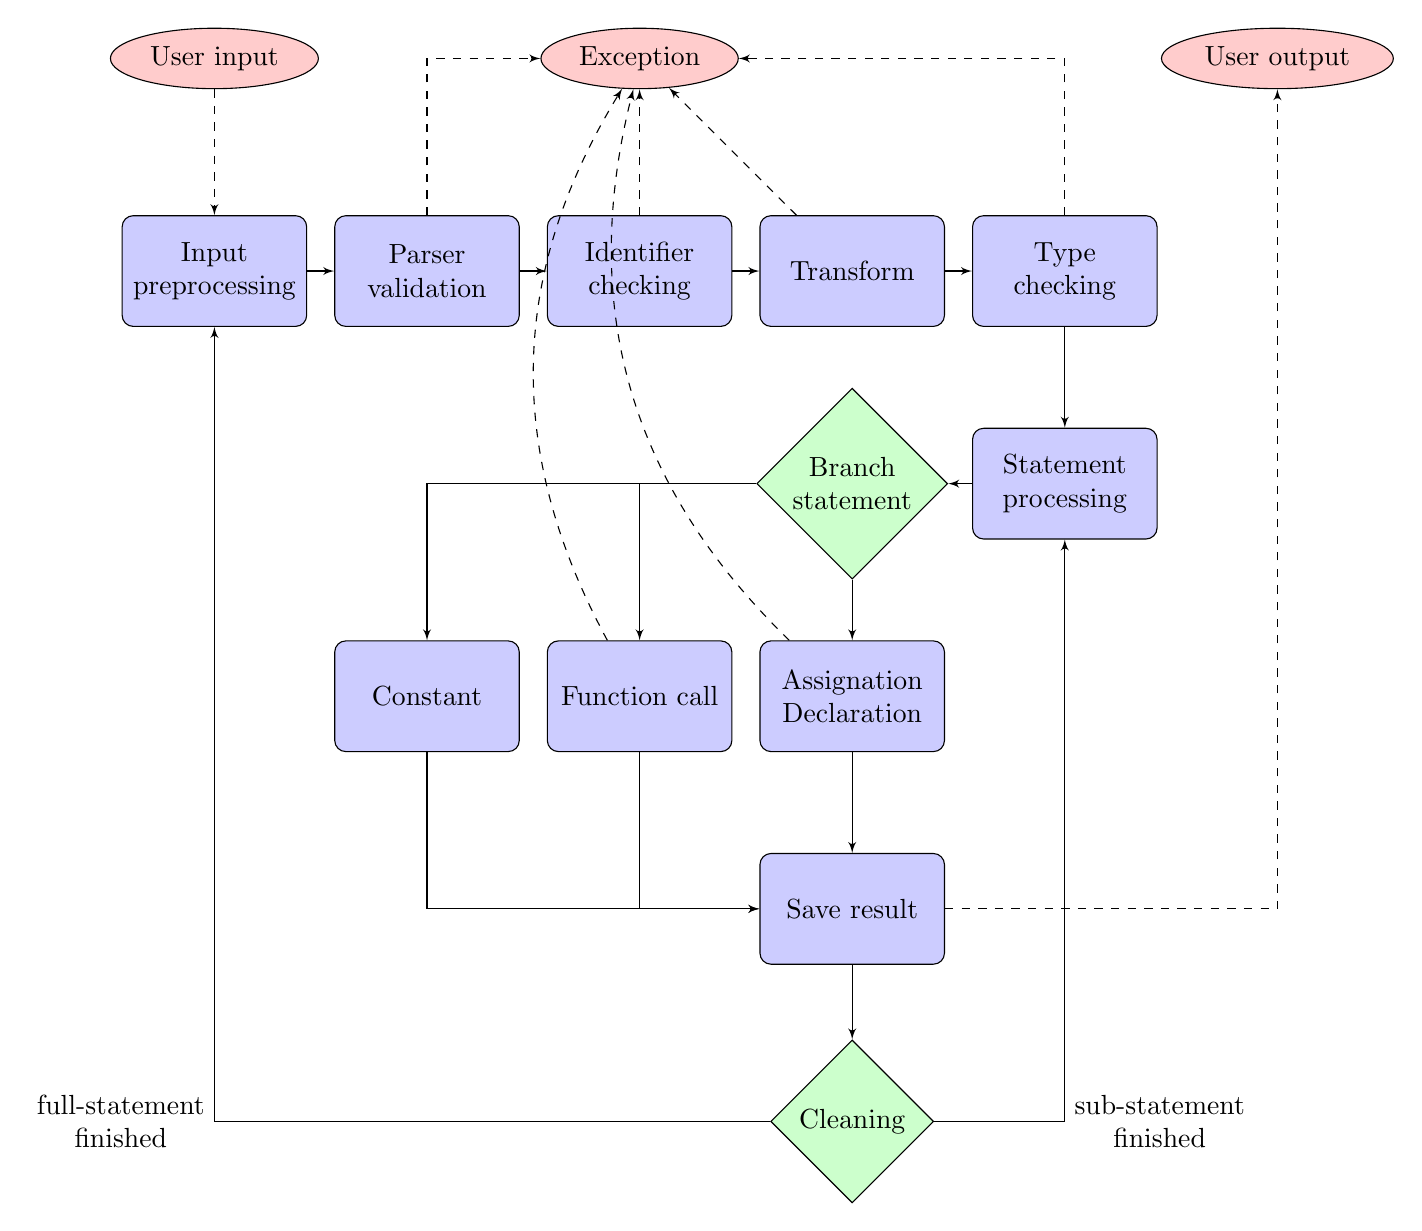
\begin{tikzpicture}[node distance = 2.7cm,auto]
					\node[cloud] (input) {User input};
					\node[block,below of=input] (preprocessor) {Input preprocessing};
					\node[block,right of=preprocessor] (parser) {Parser validation};
					\node[block,right of=parser] (identifier) {Identifier checking};
					\node[cloud,above of=identifier] (exception) {Exception};
					\node[block,right of=identifier] (transformation) {Transform};
					\node[block,right of=transformation] (type) {Type checking};
					\node[block,below of=type] (parameter) {Statement processing};
					\node[decision,left of=parameter] (execute) {Branch statement};
					\node[block,below of=execute] (assign) {Assignation Declaration};
					\node[block,left of=assign] (function) {Function call};
					\node[block,left of=function] (constant) {Constant};
					\node[block,below of=assign] (result) {Save result};
					\node[decision,below of=result] (clean) {Cleaning};
					\node[cloud,right of=type,above of=type] (output) {User output};
					
					\path[line,dashed] (input) -- (preprocessor);
					\path[line,dashed] (parser) |- (exception);
					\path[line,dashed] (identifier) -- (exception);
					\path[line,dashed] (type) |- (exception);
					\path[line,dashed] (transformation) -- (exception);
					\path[line,dashed] (function) edge[bend left] (exception);
					\path[line,dashed] (assign) edge[bend left] (exception);
					\path[line] (preprocessor) -- (parser);
					\path[line] (parser) -- (identifier);
					\path[line] (identifier) -- (transformation);
					\path[line] (transformation) -- (type);
					\path[line] (type) -- (parameter);
					\path[line] (parameter) -- (execute);
					\path[line] (execute) -| (function);
					\path[line] (execute) -- (assign);
					\path[line] (execute) -| (constant);
					\path[line] (function) |- (result);
					\path[line] (assign) -- (result);
					\path[line] (constant) |- (result);
					\path[line] (result) -- (clean);
					\path[line] (clean) -| node[align=center,right] {sub-statement\\finished} (parameter);
					\path[line] (clean) -| node[align=center] {full-statement\\finished} (preprocessor);
					\path[line,dashed] (result) -| (output);
				\end{tikzpicture}
				\caption{Flux des données dans l'interpréteur}
			\end{figure}
			
			Détaillons chacune de ces étapes:
			\begin{enumerate}
				\item \textbf{Input preprocessing} - On récupère les entrées utilisateur dans un tampon 
				\begin{enumerate}
					\item \textbf{Trim} - On enlève tous les espaces inutiles, c'est-à-dire tous les espaces sauf ceux dans les constantes littérales de type \textit{String}, et celui qui sépare le type de l'identifiant dans les déclarations
					\item \textbf{Statement per statement} - On envoie au parser une commande à la fois (les traitements sont séparés par des ';') 
				\end{enumerate}
				\item \textbf{Parser validation} - On vérifie la syntaxe de la commande et on extrait des informations utiles pour la suite (tokens), voir section~\ref{subsec:implementation-du-parseur}
				\item \textbf{Identifier checking} - On connaît les différents identifiants présents dans la commande (noms de variable, noms de fonction), on peut tout de suite vérifier leur existance 
				\item \textbf{Transform} - On transforme la commande en arbre d'appel, plus de détails dans la section~\ref{subsec:regles-de-transformation}
				\item \textbf{Type checking} - On vérifie la concordance des types (statique), plus de détails dans la section~\ref{subsubsec:verification-des-types}
				\item \textbf{Statement processing} - La commande a été décomposée en plusieurs sous-traitements (arbre d'appel, \ref{subsubsec:arbre-d-appel-des-traitements}), on effectue d'abord les feuilles avant de remonter
				\begin{enumerate}
					\item \textbf{Branch statement} - On sélectionne le bon traitement en fonction de son type
					\begin{itemize}
						\item \textbf{Constant} - On créé une variable temporaire avec la valeur de la constante, voir section~\ref{subsubsec:table-des-temporaires}
						\item \textbf{Function call} - On appelle la fonction et on sauve son résultat dans une variable temporaire
						\item \textbf{Assignation} - On assigne une valeur à une variable, voir section~\ref{subsubsec:table-des-variables}
						\item \textbf{Declaration} - Pareil que l'assignation, mais avec création de l'identifiant au préalable 
					\end{itemize}
					\item \textbf{Save result} - On transforme l'arbre d'appel avec les nouvelles valeurs/variables. Si c'est la fin de la commande, on indique à l'utilisateur que le résultat de la commande est prêt
					\item \textbf{Cleaning} - On supprime les variables temporaires qui ne sont plus utiles. Si c'était un sous-traitement, on passe au prochain sous-traitement (6), sinon on passe à la prochaine commande (1)
				\end{enumerate}
			\end{enumerate}
			
		\subsection{Implémentation du parseur}
			\label{subsec:implementation-du-parseur}
			Boost.Spirit toussa todo blabla ...
		
		\subsection{Mémoire virtuelle} 
			\label{subsec:memoire-virtuelle}
			Dans le flux de données, certaines étapes nécessitent l'utilisation d'une mémoire afin de gérer les variables (temporaires ou non). Dans cette section nous allons préciser comment cela va être géré.\\
			
			Chaque type du langage possède son pendant en C++, voici un tableau résumant cela:\\
			
			\begin{tabular}{r|l}
				Type & Equivalent C++\\ \hline\hline
				\texttt{Boolean} & \texttt{bool}\\
				\texttt{Integer} & \texttt{int}\\
				\texttt{Float} & \texttt{float}\\
				\texttt{String} & \texttt{std::string}\\
				\texttt{Number} & voir section~\ref{subsubsec:number-edge-et-vertex}\\
				\texttt{Array} & voir section~\ref{subsubsec:tableau-dynamique-heterogene}\\
				\texttt{Graph} & voir section~\textcolor{red}{ajouter ref}\\
				\texttt{Vertex} & voir section~\ref{subsubsec:number-edge-et-vertex}\\
				\texttt{Edge} & voir section~\ref{subsubsec:number-edge-et-vertex}
			\end{tabular}
			
			\subsubsection{Table des variables}
				\label{subsubsec:table-des-variables}
			
			\subsubsection{Table des temporaires}
				\label{subsubsec:table-des-temporaires}
				
			\subsubsection{Tableau dynamique hétérogène}
				\label{subsubsec:tableau-dynamique-heterogene}
				Le tableau dynamique hétérogène (TDH dans la suite de cette section) pose un gros problème majeur: le C++ est un langage fortement typé. Cependant plusieurs solutions s'offrent à nous pour créer un TDH:
				
				\begin{enumerate}
					\item Un \texttt{std::vector<boost::any>} (\texttt{std::any} étant prévu pour C++17)
					\item Un \texttt{std::vector<std::pair<std::type\_index, void*> >}
					\item Un \texttt{std::vector<std::pair<TypeEnum, void*> >}
				\end{enumerate}
				
				La solution (1) est sans doute la plus propre ainsi que la plus facile, cependant elle ajoute une dépendance avec Boost et elle partage plusieurs problèmes avec la solution (2) que l'on va voir tout de suite.\\
				
				La solution (2) utilise un mécanisme de C++ (l'opérateur \texttt{typeid}) afin de savoir quel est le type réel caché derrière le \texttt{void*}, cela permet un code assez générique. Cependant pour chaque valeur, on doit attacher un objet \texttt{std::type\_index} (lui-même composé d'un \texttt{std::type\_info}), et faire des appels à \texttt{typeid}, cela ajoute un surcoût en temps et en mémoire par rapport à la solution (3).\\
				
				La solution (3) est donc celle retenue pour implémenter un TDH. On créé simplement une énumération contenant les types acceptés dans le TDH, et chaque \texttt{void*} est associé à une valeur de cette énumération.
				
				\begin{lstlisting}[language=C++]
					class Array {
					public:
						enum class Type { Boolean, Integer, String /*, ...*/ };
						typedef std::pair<Type, void*> value_type;
						
						// constructeur de copie, etc.
						// ...
						
						~Array() {
							for(value_type& value : values) {
								switch(value.first) {
									case Type::Boolean:
										delete (bool*)value.second;
										break;
									case Type::Integer:
										delete (int*)value.second;
										break;
									case Type::String:
										delete (std::string*)value.second;
										break;
									// ...
								}
							}
						}
						
						size_t size() const {
							return values.size();
						}
						
						void add(int *value) { 
							// value doit provenir d'un 'new'
							values.push_back(std::make_pair(Type::Integer, (void*)value));
						}
						
						void add(int value) {
							add(new int(value));
						}
						// ...
						
						Type typeOf(size_t i) const {
							return values.at(i).first;
						}
						
						int getInteger(size_t i) const {
							if(typeOf(i) != Type::Integer)
								throw /* cast exception */;
							return *(int*)values.at(i).second;
						}
						// ...
						
					private:
					
						std::vector<value_type> values;
					};
				\end{lstlisting}
				
				Cette solution est assez verbeuse, cependant la complexité en temps et en mémoire est très bonne. En ce qui concerne les \texttt{delete}, il est obligatoire de faire le cast avant, sinon le destructeur de l'objet détruit n'est pas appelé.\\
				
				Evidemment l'utilisateur du TDH est obligé de faire des \texttt{switch/if-else} dans son code, cependant ce problème vaut pour chacune des trois solutions et est inhérent au C++.  
				
			\subsubsection{Number, Edge et Vertex}
				\label{subsubsec:number-edge-et-vertex}
				Number
				Optional
				Vertex
				Edge
				
		\subsection{Table des fonctions}
			Dans le flux de données, l'étape \textit{Function call} nécessite d'appeler, d'exécuter et de récupérer le résultat d'une fonction. Dans cette section nous allons préciser comment cela va être fait.
			
			\subsubsection{Interfaçage}
			\label{subsubsec:interfacage}
			
			\subsection{Règles de transformation}
			\label{subsec:regles-de-transformation}
			Dans cette section nous allons préciser les règles de transformation de l'étape \textit{Transform} du flux de données, ainsi que ce que cela va apporter.
			
			\subsubsection{Arbre d'appel des traitements}
			\label{subsubsec:arbre-d-appel-des-traitements}
			
			\subsubsection{Vérification des types}
			\label{subsubsec:verification-des-types}
			
			\subsection{Exemples}
	
	\section{Annexes}
	
	\begin{thebibliography}{9}
		\bibitem{vutbr.cz} 
		Faculty of Technology, Brno University of Technology, Réplublique tchèque,\\ \url{http://www.fit.vutbr.cz/study/courses/APR/public/ebnf.html}
	\end{thebibliography}			

\end{document}
